Cambio de dirección que experimenta una onda al pasar de un medio a otro con diferenta velocidad de propagación. Esto ocurre porque la onda cambia de velocidad al entrar en el nuevo medio, lo que provoca que se desvíe de su trayectoria original.

Cada medio, debido a sus propiedades físicas, tiene una velocidad de propagación diferente. Cuando las ondas interactuan con cada medio, su trayectoria está condicionada por la velocidad con la que se mueve dentro de se medio.

\begin{figure}
  \centering
  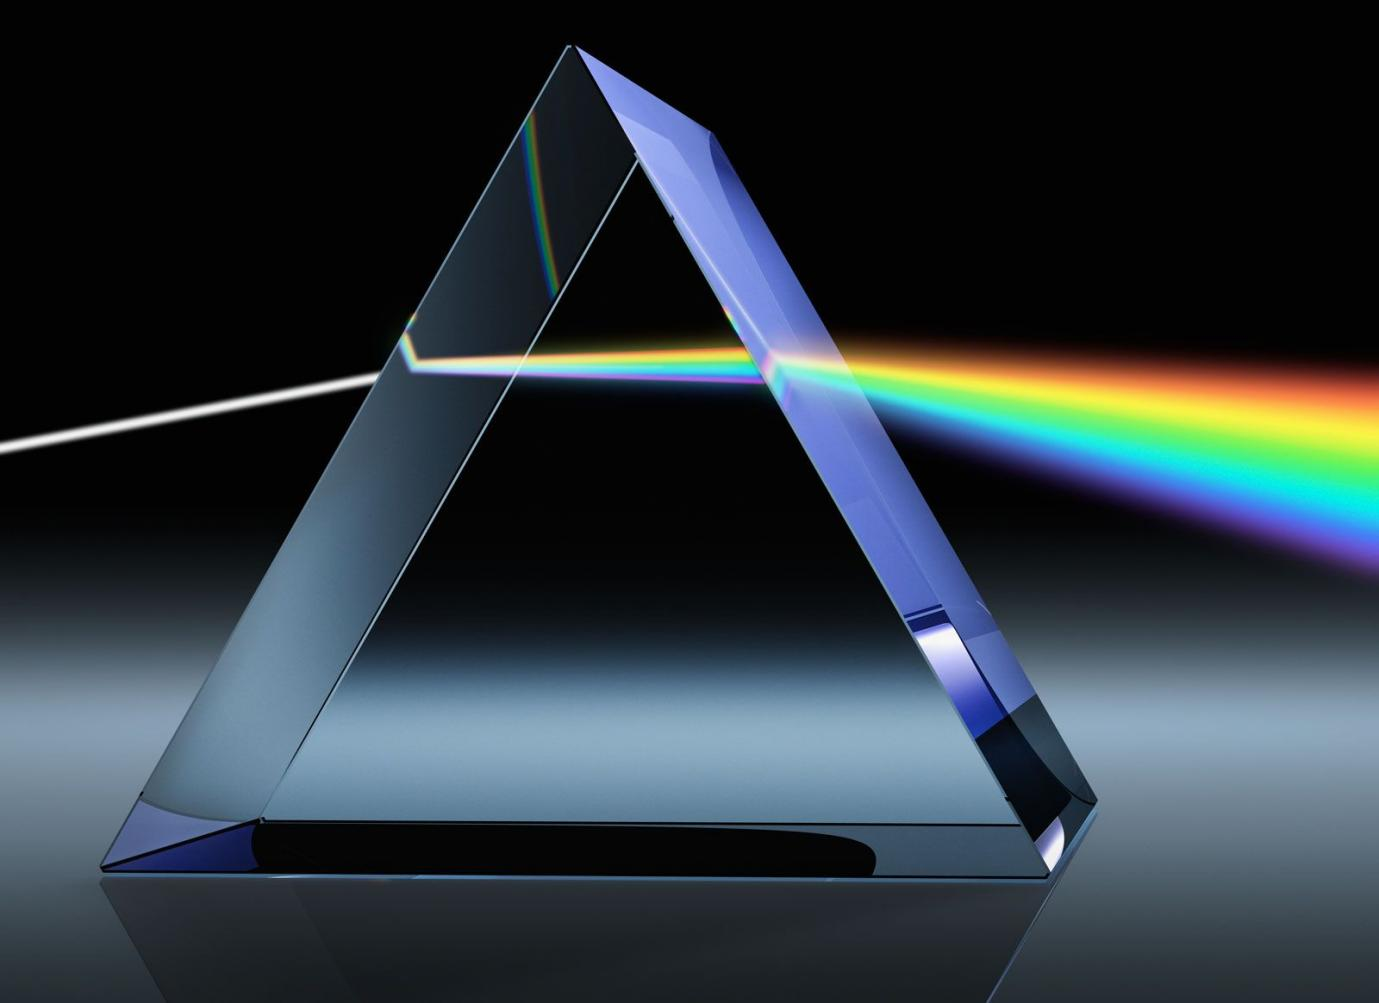
\includegraphics[scale=0.5]{imagenes/prisma.png}
  \caption{Refracción en un prisma\cite{cstmglassprism}}
\end{figure}

La refracción ocurre todo el tiempo. Se usa para enfocar la luz y crear imagenes claras mediante lentes de gafas, cámaras telescopios, microscopios y otros. Los arcoiris ocurren cuando la luz se refracta en las gotas de lluvia. Los objetos en el agua parecen estar doblados por efecto de la refracción.

Un gran ejemplos son los prismas hechos cristal o vidrio. La luz blanca, que es la combinación de todos los colores, al pasar a través del prisma se descompone en un espectro de colores como un arcoiris. Esto se debe a la distinta longitud de onda de los colores en el rango de luz visible.
